% \documentclass[9pt,t]{beamer}
\usefonttheme{professionalfonts}
\usefonttheme{serif}
\PassOptionsToPackage{pdfpagemode=FullScreen}{hyperref}
\PassOptionsToPackage{usenames,dvipsnames}{color}
% \DeclareGraphicsRule{*}{mps}{*}{}
\usepackage{linalgjh}
\usepackage{present}
\usepackage{directories}
\usepackage{xr}\externaldocument{\jcdir jc2} % read refs from .aux file
\usepackage{catchfilebetweentags}
\usepackage{etoolbox} % from http://tex.stackexchange.com/questions/40699/input-only-part-of-a-file-using-catchfilebetweentags-package
\makeatletter
\patchcmd{\CatchFBT@Fin@l}{\endlinechar\m@ne}{}
  {}{\typeout{Unsuccessful patch!}}
\makeatother

\usepackage{polynom}  % for polynomial long division

\mode<presentation>
{
  \usetheme{boxes}
  \setbeamercovered{invisible}
  \setbeamertemplate{navigation symbols}{} 
}
\addheadbox{filler}{\ }  % create extra space at top of slide 
\hypersetup{colorlinks=true,linkcolor=blue} 

\title[Similarity] % (optional, use only with long paper titles)
{Five.II Similarity}

\author{\textit{Linear Algebra} \\ {\small Jim Hef{}feron}}
\institute{
  \texttt{https://hefferon.net/linearalgebra}\\[0.25ex]
  \texttt{http://joshua.smcvt.edu/linearalgebra}
}
\date{}


\subject{Similarity}
% This is only inserted into the PDF information catalog. Can be left
% out. 

\begin{document}
\begin{frame}
  \titlepage
\end{frame}



\section{Definition and Examples}
% =============================================
\begin{frame}
\vspace*{-2ex}
\ExecuteMetaData[\jcdir jc2.tex]{SimilarityMotiviation0}  
\pause  
\ExecuteMetaData[\jcdir jc2.tex]{SimilarityMotiviation1}  
\end{frame}




% ..... Five.II.1 .....
\begin{frame}{Similar matrices}
\df[df:Similar]
\ExecuteMetaData[\jcdir jc2.tex]{df:Similar}  

\ex
Consider the derivative map $\map{d/dx}{\polyspace_2}{\polyspace_2}$.
Fix the basis $B=\sequence{1,x,x^2}$ 
and the basis $D=\sequence{1,1+x,1+x+x^2}$.
In this arrow diagram we will first get $T$, and then calculate $\hat{T}$ 
from it.
\begin{equation*}
  \begin{CD}
    V_{\wrt{B}}                   @>t>T>        V_{\wrt{B}}       \\
    @V{\scriptstyle\identity} VV              @V{\scriptstyle\identity} VV \\
    V_{\wrt{D}}                   @>t>\hat{T}>        V_{\wrt{D}}
  \end{CD}
\end{equation*}
\pause
The action of $d/dx$ on the 
elements of the basis $B$ is $1\mapsto 0$, $x\mapsto 1$, and $x^2\mapsto 2x$.
\begin{equation*}
  \rep{\frac{d}{dx}(1)}{B}=\colvec{0 \\ 0 \\ 0}
  \hspace{0.8em}
  \rep{\frac{d}{dx}(x)}{B}=\colvec{1 \\ 0 \\ 0}
  \hspace{0.8em}
  \rep{\frac{d}{dx}(x^2)}{B}=\colvec{0 \\ 2 \\ 0}
\end{equation*}
\end{frame}
\begin{frame}
So we have this matrix representation of the map.
\begin{equation*}
  T=\rep{\frac{d}{dx}}{B,B}=
  \begin{mat}
    0 &1 &0 \\
    0 &0 &2 \\
    0 &0 &0
  \end{mat}
\end{equation*}
\pause
The matrix changing bases from $B$ to $D$ is $\rep{\identity}{B,D}$.
We find these by eye
\begin{equation*}
  \rep{\identity(1)}{D}=\colvec{1 \\ 0 \\ 0}
  \quad
  \rep{\identity(x)}{D}=\colvec{-1 \\ 1 \\ 0}
  \quad
  \rep{\identity(x^2)}{D}=\colvec{0 \\ -1 \\ 1}
\end{equation*}
to get this.
\begin{equation*}
  P=
  \begin{mat}
    1 &-1 &0  \\
    0 &1  &-1 \\
    0 &0  &1
  \end{mat}
  \qquad
  P^{-1}=
  \begin{mat}
    1 &1  &1  \\
    0 &1  &1 \\
    0 &0  &1
  \end{mat}
\end{equation*}
Now, by following the arrow diagram we have $\hat{T}=PTP^{-1}$.
\begin{equation*}
  \hat{T}=
  \begin{mat}
    0 &1 &-1 \\
    0 &0 &2  \\
    0 &0 &0
  \end{mat}
\end{equation*}
\end{frame}
\begin{frame}
To check that, and to underline what the arrow diagram says 
\begin{equation*}
  \begin{CD}
    V_{\wrt{B}}                   @>t>T>        V_{\wrt{B}}       \\
    @V{\scriptstyle\identity} VV              @V{\scriptstyle\identity} VV \\
    V_{\wrt{D}}                   @>t>\hat{T}>        V_{\wrt{D}}
  \end{CD}
\end{equation*}
we calculate $\hat{T}$ directly.
The effect of the map on the basis elements is 
$d/dx(1)=0$, $d/dx(1+x)=1$, and $d/dx(1+x+x^2)=1+2x$.
Representing of those with respect to $D$
\begin{equation*}
  \rep{0}{D}=\colvec{0 \\ 0 \\ 0}
  \quad
  \rep{1}{D}=\colvec{1 \\ 0 \\ 0}
  \quad
  \rep{1+2x}{D}=\colvec{-1 \\ 2 \\ 0}
\end{equation*}
gives the same matrix $\hat{T}=\rep{d/dx}{D,D}$ as above.
\end{frame}
\begin{frame}
The definition doesn't require that we consider the underlying maps.
We can just multiply matrices.  

\ex
Where 
\begin{equation*}
  T=
  \begin{mat}
    0 &-1 &-2 \\
    2 &3 &2   \\
    4 &5 &2
  \end{mat}
  \qquad
  P=
  \begin{mat}
    1 &1 &0 \\
   -1 &1 &0   \\
    0 &0 &3
  \end{mat}
\end{equation*}
(note that $P$ is nonsingular) we can compute this $\hat{T}=PTP^{-1}$.
\begin{equation*}
  \hat{T}=
  \begin{mat}
    2   &0   &0 \\
    3   &1   &4/3 \\
   27/2 &3/2 &2
  \end{mat}
\end{equation*}

\pause
\ex[ex:OnlyZeroSimToZero]
\ExecuteMetaData[\jcdir jc2.tex]{ex:OnlyZeroSimToZero}  
\end{frame}



\begin{frame}{Similarity is an equivalence}
\nearbyexercise{exer:SimIsEquivRel} checks that
similarity is an equivalence relation.

\pause
Since matrix similarity is a special case of matrix equivalence, 
if two matrices are similar then they are matrix equivalent.
What about the converse:~must any two matrix equivalent square matrices be 
similar?
No; the matrix equivalence class
of an identity consists of all nonsingular matrices of that size while the 
prior example shows that an identity matrix is alone in its similarity
class. 

\pause
So some matrix equivalence classes
split into two or more similarity classes\Dash similarity gives a finer
partition than does equivalence.
This pictures some matrix equivalence classes subdivided into
similarity classes.
\centergraphic{\jcmpdir ch5.4} 

\pause
We naturally want a canonical form to represent the similarity classes.
Some classes, but not all,
are represented by a diagonal form.
\end{frame}




% ..... Five.II.2 .....
\section{Diagonalizability}
\begin{frame}
\df[df:Diagonalizable]
\ExecuteMetaData[\jcdir jc2.tex]{df:Diagonalizable}  

\ex
This matrix
\begin{equation*}
  \begin{mat}
    6 &-1  &-1 \\
    2 &11  &-1 \\
   -6 &-5  &7
  \end{mat}
\end{equation*}
is diagonalizable by using this
\begin{equation*}
  P=
  \begin{mat}
    1/2 &1/4  &1/4 \\
   -1/2 &1/4  &1/4 \\
   -1/2 &-3/4 &1/4
  \end{mat}
  \quad
  P^{-1}=
  \begin{mat}
    1 &-1 &0 \\
    0 &1 &-1 \\
    2 &1 &1
  \end{mat}
\end{equation*}
to get this $D=PSP^{-1}$.
\begin{equation*}
  D=
  \begin{mat}
    4 &0 &0 \\
    0 &8 &0 \\
    0 &0 &12
  \end{mat}
\end{equation*}
\end{frame}
\begin{frame}
\ex  
\ExecuteMetaData[\jcdir jc2.tex]{ex:NotDiagonalizable}  
\end{frame}




\begin{frame}
\lm[lm:DiagIffBasisOfEigens]
\ExecuteMetaData[\jcdir jc2.tex]{lm:DiagIffBasisOfEigens}  

\pause
\pf
\ExecuteMetaData[\jcdir jc2.tex]{pf:DiagIffBasisOfEigens}  
\qed
\end{frame}

\begin{frame}
\ex
This matrix is not diagonal
\begin{equation*}
  T=
  \begin{mat}
    4  &1  \\
    0  &-1
  \end{mat}
\end{equation*}
but we can
find a diagonal matrix similar to it, by finding an appropriate basis.

\pause
Suppose that $T=\rep{t}{\stdbasis_2,\stdbasis_2}$ for $\map{t}{\Re^2}{\Re^2}$.
We will find a basis $B=\sequence{\vec{\beta}_1,\vec{\beta}_2}$ giving a 
diagonal representation.
\begin{equation*}
  D=\rep{t}{B,B}=
  \begin{mat}
    \lambda_1  &0 \\
    0    &\lambda_2
  \end{mat}
\end{equation*}
Here is the arrow diagram.
\begin{equation*}
  \begin{CD}
    V_{\wrt{\stdbasis_2}}            @>t>T>        V_{\wrt{\stdbasis_2}}       \\
    @V{\scriptstyle\identity} VV              @V{\scriptstyle\identity} VV \\
    V_{\wrt{B}}                   @>t>D>        V_{\wrt{B}}
  \end{CD}
\end{equation*}
\end{frame}
\begin{frame}
We want $\lambda_1$ and $\lambda_2$ making these true.
\begin{equation*}
  \begin{mat}
    4  &1  \\
    0  &-1    
  \end{mat}
  \vec{\beta}_1
  =\lambda_1\cdot\vec{\beta}_1
  \qquad
  \begin{mat}
    4  &1  \\
    0  &-1    
  \end{mat}
  \vec{\beta}_2
  =\lambda_2\cdot\vec{\beta}_2
\end{equation*}
More precisely, 
we want all scalars $x\in\C$ such that this system
\begin{equation*}
  \begin{mat}
    4  &1  \\
    0  &-1    
  \end{mat}
  \colvec{b_1 \\ b_2}
  =x\cdot\colvec{b_1 \\ b_2}
\end{equation*}
has solutions $b_1,b_2\in\C$ that are not both zero
(the zero vector is not an element of any basis).
% \end{frame}
% \begin{frame}

\pause
Rewrite that as a linear system.
\begin{equation*}
  \begin{linsys}{2}
    (4-x)\cdot b_1 &+ &b_2             &= &0 \\
                   &  &(-1-x)\cdot b_2 &= &0 
  \end{linsys}
  % \tag{$*$}
\end{equation*}
One solution is $\lambda_1=-1$, associated with those
$(b_1,b_2)$ such that $b_1=(-1/5)b_2$.
The other solution is $\lambda_2=4$, associated with the
$(b_1,b_2)$ such that
$b_2=0$.
\end{frame}
\begin{frame}
Thus the original matrix  
\begin{equation*}
  T=
  \begin{mat}[r]
    4  &1  \\
    0  &-1
  \end{mat}
\end{equation*}
is diagonalizable to
\begin{equation*}
  D=
  \begin{mat}[r]
    -1  &0  \\
    0  &4
  \end{mat}
\end{equation*}
where this is a basis.
\begin{equation*}
  B=\sequence{\colvec[r]{-1 \\ 5},
              \colvec{1 \\ 0}}
\end{equation*}
\end{frame}




% ..... Five.II.3 .....
\section{Eigenvalues and Eigenvectors}
\begin{frame}{Eigenvalues and eigenvectors}
\df[def:Eigen]
\ExecuteMetaData[\jcdir jc2.tex]{df:Eigen}  

\pause
\df[df:EigenOfMatrix]
\ExecuteMetaData[\jcdir jc2.tex]{df:EigenOfMatrix}  

\ex
The matrix
\begin{equation*}
  D=
  \begin{mat}
    4  &0 \\
    0  &2  
  \end{mat}
\end{equation*}
has an eigenvalue $\lambda_1=4$ and a second eigenvalue $\lambda_2=2$.
The first is true because an associated eigenvector is
$\vec{e_1}$
\begin{equation*}
  \begin{mat}
    4  &0 \\
    0  &2  
  \end{mat}
  \colvec{1 \\ 0}
  =
  4\cdot\colvec{1 \\ 0}  
\end{equation*}
and similarly for the second an associated eigenvector
is $e_2$.
\begin{equation*}
  \begin{mat}
    4  &0 \\
    0  &2  
  \end{mat}
  \colvec{0 \\ 1}
  =
  2\cdot\colvec{0 \\ 1}  
\end{equation*}
\end{frame}
\begin{frame}
If we think of that matrix as representing a transformation of the plane,
the transformation acts on those vectors in a particularly simple way, 
by rescaling.

But note that not every vector is simply rescaled.
\begin{equation*}
  \begin{mat}
    4  &0 \\
    0  &2  
  \end{mat}
  \colvec{1 \\ 1}
  =\colvec{4 \\ 2}
  \neq
  x\cdot\colvec{1 \\ 1}  
\end{equation*}
Those that are rescaled, the eigenvectors, are special.
\end{frame}




\begin{frame}{Computing eigenvalues and eigenvectors}
\ex
We will find the eigenvalues and associated eigenvectors of this matrix.
\begin{equation*}
  T=
  \begin{mat}
    0 &5 &7 \\
   -2 &7 &7 \\
   -1 &1 &4
  \end{mat}
\end{equation*}
We want to find scalars~$x$ such that $T\vec{\zeta}=x\vec{\zeta}$ for 
some nonzero $\vec{\zeta}$.
Bring the terms to the left side.
\begin{equation*}
  \begin{mat}
    0 &5 &7 \\
   -2 &7 &7 \\
   -1 &1 &4
  \end{mat}
  \colvec{z_1 \\ z_2 \\ z_3}
  -x\colvec{z_1 \\ z_2 \\ z_3}
  =\colvec{0 \\ 0 \\ 0}
\end{equation*}
and factor out the vector.
\begin{equation*}
  \begin{mat}
    0-x &5   &7 \\
   -2   &7-x &7 \\
   -1   &1   &4-x
  \end{mat}
  \colvec{z_1 \\ z_2 \\ z_3}
  =
  \colvec{0 \\ 0 \\ 0}
  \tag{$*$}
\end{equation*}
This homogeneous system has nonzero solutions if and only if the 
matrix is singular, that is, has a determinant of zero.
\end{frame}
\begin{frame}
Some computation gives the determinant and its factors.
\begin{align*}
  0&=
  \begin{vmat}
    0-x &5   &7 \\
   -2   &7-x &7 \\
   -1   &1   &4-x
  \end{vmat}          \\
  &=
  x^3 - 11x^2 + 38x - 40
  =(x - 5)(x - 4)(x - 2)
\end{align*}
So the eigenvalues are $\lambda_1=5$, $\lambda_2=4$, and $\lambda_3=2$.

\pause
To find the eigenvectors associated with the eigenvalue of $5$, 
specialize equation~($*$) for $x=5$.
\begin{equation*}
  \begin{mat}
   -5   &5   &7 \\
   -2   &2   &7 \\
   -1   &1   &-1
  \end{mat}
  \colvec{z_1 \\ z_2 \\ z_3}
  =
  \colvec{0 \\ 0 \\ 0}
\end{equation*}
Gauss's Method gives this solution set; its nonzero elements are the 
eigenvectors.
\begin{equation*}
  V_5=\set{\colvec{1 \\ 1 \\ 0}z_2\suchthat z_2\in\C}
\end{equation*}
\end{frame}
\begin{frame}
Similarly, to find the eigenvectors associated with the eigenvalue of~$4$, 
specialize equation~($*$) for $x=4$.
\begin{equation*}
  \begin{mat}
   -4   &5   &7 \\
   -2   &3   &7 \\
   -1   &1   &0
  \end{mat}
  \colvec{z_1 \\ z_2 \\ z_3}
  =
  \colvec{0 \\ 0 \\ 0}
\end{equation*}
Gauss's Method gives this.
\begin{equation*}
  V_4=\set{\colvec{-7 \\ -7 \\ 1}z_3\suchthat z_3\in\C}
\end{equation*}
\pause
Specializing~($*$) for~$x=2$
\begin{equation*}
  \begin{mat}
   -2   &5   &7 \\
   -2   &5   &7 \\
   -1   &1   &2
  \end{mat}
  \colvec{z_1 \\ z_2 \\ z_3}
  =
  \colvec{0 \\ 0 \\ 0}
\end{equation*}
gives this.
\begin{equation*}
  V_2=\set{\colvec{1 \\ -1 \\ 1}z_3\suchthat z_3\in\C}
\end{equation*}
\end{frame}




% --

\begin{frame}
\ex
To find the eigenvalues and associated eigenvectors for the matrix
\begin{equation*}
  T=
  \begin{mat}
    3  &1  \\
    1  &3
  \end{mat}
\end{equation*}
start with this equation.
\begin{equation*}
  \begin{mat}
    3  &1  \\
    1  &3    
  \end{mat}
  \colvec{b_1 \\ b_2}
  =x\colvec{b_1 \\ b_2}
  \quad\Longrightarrow\quad
  \begin{mat}
    3-x  &1  \\
    1    &3-x    
  \end{mat}
  \colvec{b_1 \\ b_2}
  =\colvec{0 \\ 0}
  \tag{$*$}
\end{equation*}
\pause
That system
has a nontrivial solution if this determinant is nonzero.
\begin{equation*}
  \begin{vmat}
    3-x  &1  \\
    1    &3-x
  \end{vmat}
  =x^2-6x+8
  =(x-2)(x-4)
\end{equation*}
\pause
First take the $x=2$ version of~($*$).
\begin{equation*}
  \begin{linsys}{2}
    1\cdot b_1 &+ &b_2        &= &0 \\
    b_1        &+ &1\cdot b_2 &= &0 
  \end{linsys}
  \quad\Longrightarrow\quad
  V_2=\set{\colvec{b_1 \\ b_2}\suchthat \text{$b_1=-b_2$ where $b_2\in\C$}}
\end{equation*}
Solving the second system is just as easy.
\begin{equation*}
  \begin{linsys}{2}
    -1\cdot b_1 &+ &b_2        &= &0 \\
    b_1        &- &1\cdot b_2 &= &0 
  \end{linsys}
  \quad\Longrightarrow\quad
  V_4=\set{\colvec{b_1 \\ b_2}\suchthat \text{$b_1=b_2$ where $b_2\in\C$}}
\end{equation*}
\end{frame}




\begin{frame}
\ex 
If the matrix is upper diagonal or lower diagonal
\begin{equation*}
  T=
  \begin{mat}
    2 &1 &0 \\
    0 &3 &1 \\
    0 &0 &2
  \end{mat}
\end{equation*}
then the polynomial is easy to factor.
\begin{equation*}
  0=
  \begin{vmat}
    2-x &1   &0 \\
    0   &3-x &1 \\
    0   &0   &2-x
  \end{vmat}
  =(3-x)(2-x)^2
\end{equation*}
\pause
These are the solutions for $\lambda_1=3$.
\begin{equation*}
  \begin{mat}
    -1  &1   &0 \\
    0   &0   &1 \\
    0   &0   &-1
  \end{mat}
  \colvec{z_1 \\ z_2 \\ z_3}
  =
  \colvec{0 \\ 0 \\ 0}
  \quad\Longrightarrow\quad
  V_3=\set{\colvec{1 \\ 1 \\ 0}z_2\suchthat z_2\in\C}
\end{equation*}
These are for $\lambda_2=2$.
\begin{equation*}
  \begin{mat}
    0  &1   &0 \\
    0   &1   &1 \\
    0   &0   &0
  \end{mat}
  \colvec{z_1 \\ z_2 \\ z_3}
  =
  \colvec{0 \\ 0 \\ 0}
  \quad\Longrightarrow\quad
  V_2=\set{\colvec{1 \\ 0 \\ 0}z_1\suchthat z_1\in\C}
\end{equation*}  
\end{frame}


\begin{frame}
Matrices that are similar have the same eigenvalues, but
needn't have the same eigenvectors.

\ex
These two are similar 
\begin{equation*}
  T=
  \begin{mat}
    4 &0 &0 \\
    0 &8 &0 \\
    0 &0 &12
  \end{mat}
  \qquad
  S=
  \begin{mat}[r]
    6 &-1  &-1 \\
    2 &11  &-1 \\
   -6 &-5  &7
  \end{mat}
\end{equation*}
since $S=PTP^{-1}$ for this $P$.
\begin{equation*}
  P=
  \begin{mat}[r]
    1 &-1 &0 \\
    0 &1 &-1 \\
    2 &1 &1
  \end{mat}
  \qquad
  P^{-1}=
  \begin{mat}[r]
    1/2 &1/4  &1/4 \\
   -1/2 &1/4  &1/4 \\
   -1/2 &-3/4 &1/4
  \end{mat}
\end{equation*}
For the first matrix
\begin{equation*}
  \colvec{1 \\ 0 \\ 0}
\end{equation*}
is an eigenvector associated with the eigenvalue~$4$ but 
that does not hold for the second matrix.
\end{frame}
% \begin{frame}
% \noindent Suppose that $\map{t}{\C^3}{\C^3}$ is
% represented by $T$ with respect to the standard basis.
% Then this is the action of $t$.
% \begin{equation*}
%   \colvec{x \\ y \\ z}\mapsunder{t}\colvec{4x \\ 8y  \\ 12z}
% \end{equation*}
% \pause
% By eye we see that three 
% eigenvalues of~$t$ are $\lambda_1=4$, $\lambda_2=8$, and~$\lambda_3=12$.
% For instance this holds.
% \begin{equation*}
%   T\cdot\colvec{1 \\ 0 \\ 0}
%   =\begin{mat}
%     4 &0 &0 \\
%     0 &8 &0 \\
%     0 &0 &12
%   \end{mat}\colvec{1 \\ 0 \\ 0}
%   =4\cdot\colvec{1 \\ 0 \\ 0}
% \end{equation*}
% \end{frame}
% \begin{frame}
% Contrast that with $S=PTP^{-1}$, which represents the same function, but 
% with respect to a different basis.  
% \begin{equation*}
%   \begin{CD}
%     V_{\wrt{\stdbasis_3}}            @>t>T>        V_{\wrt{\stdbasis_3}}       \\
%     @V{\scriptstyle\identity} VV              @V{\scriptstyle\identity} VV \\
%     V_{\wrt{B}}                   @>t>S>        V_{\wrt{B}}       
%   \end{CD}
% \end{equation*}
% We can easily find the basis~$B$.
% Since $P^{-1}=\rep{\identity}{B,\stdbasis_3}$, its first column is 
% $\rep{\identity(\vec{\beta}_1)}{\stdbasis_3}=\rep{\vec{\beta}_1}{\stdbasis_3}$.
% With respect to the standard basis any vector is represented by itself 
% so the first basis element $\vec{\beta}_1$ is the first column of $P^{-1}$.
% The same goes for the other two columns.
% \begin{equation*}
%   B=\sequence{\colvec[r]{1/2 \\ -1/2 \\ -1/2},
%               \colvec[r]{1/4 \\ 1/4 \\ -3/4},
%               \colvec[r]{1/4 \\ 1/4 \\ 1/4}}
% \end{equation*}
% \end{frame}
% \begin{frame}
% % We know that the transformation~$t$ has eigenvalues of $4$, $8$, and~$12$.
% % For instance $t(\vec{e}_1)=4\vec{e}_1$.
% Now, since each represents the transformation~$t$, the matrices~$T$ and $S$
% reflect the same action $\vec{e}_1\mapsto4\vec{e}_1$.
% \begin{align*}
%   &\rep{t}{\stdbasis_3,\stdbasis_3}\cdot\rep{\vec{e}_1}{\stdbasis_3}
%     =T\cdot\rep{\vec{e}_1}{\stdbasis_3}                
%     =4\cdot\rep{\vec{e}_1}{\stdbasis_3}                  \\               
%     &\rep{t}{B,B}\cdot\rep{\vec{e}_1}{B}
%     =S\cdot\rep{\vec{e}_1}{B}                                 
%     =4\cdot\rep{\vec{e}_1}{B}
% \end{align*}
% But, while in the two equations the $4$'s are the same, the vectors
% representations are not. 
% \begin{align*}
%     T\cdot\rep{\vec{e}_1}{\stdbasis_3}
%     =T\colvec{1 \\ 0 \\ 0}
%     &=4\cdot\colvec{1 \\ 0 \\ 0}                \\
%     S\cdot\rep{\vec{e}_1}{B}  
%     =S\cdot\colvec{1 \\ 0 \\ 2}
%     &=4\cdot\colvec{1 \\ 0 \\ 2}
% \end{align*}
% So the two matrices have the same eigenvalues but different eigenvectors.
% \end{frame}





\begin{frame}{Characteristic polynomial}
\df[df:CharacteristicPoly]
\ExecuteMetaData[\jcdir jc2.tex]{df:CharacteristicPoly}

\no
\ExecuteMetaData[\jcdir jc2.tex]{df:CharacteristicPolyExer}

\pause
\lm[le:MapNonTrivSpHasEigen] 
\ExecuteMetaData[\jcdir jc2.tex]{lm:MapNonTrivSpHasEigen}

\pause
\pf
\ExecuteMetaData[\jcdir jc2.tex]{pf:MapNonTrivSpHasEigen}
\qed

\pause
\re
This result is why we switched in this chapter 
from working with real number scalars
to complex number scalars.
\end{frame}




\begin{frame}{Eigenspace}
\df[df:Eigenspace]
\ExecuteMetaData[\jcdir jc2.tex]{df:Eigenspace}

\ex
Recall that this matrix has three eigenvalues, $5$, $4$, and~$2$.
\begin{equation*}
  T=
  \begin{mat}[r]
    0 &5 &7 \\
   -2 &7 &7 \\
   -1 &1 &4
  \end{mat}
\end{equation*}
Earlier, we found that these are the eigenspaces.
\begin{equation*}
    V_5=\set{\colvec[r]{1 \\ 1 \\ 0}c\suchthat c\in\C}  
    \quad
    V_4=\set{\colvec[r]{-7 \\ -7 \\ 1}c\suchthat c\in\C} 
    \quad
    V_2=\set{\colvec[r]{1 \\ -1 \\ 1}c\suchthat c\in\C}    
\end{equation*}
\end{frame}
\begin{frame}
\lm[le:EigSpaceIsSubSp] 
\ExecuteMetaData[\jcdir jc2.tex]{lm:EigSpaceIsSubSp}

\pause
\pf
\ExecuteMetaData[\jcdir jc2.tex]{pf:EigSpaceIsSubSp}
\qed
\end{frame}




\begin{frame}
\th[th:DistEValueGivesLIEvecs]
\ExecuteMetaData[\jcdir jc2.tex]{th:DistEValueGivesLIEvecs}

\pause
\pf
\ExecuteMetaData[\jcdir jc2.tex]{pf:DistEValueGivesLIEvecs0}

\pause
\ExecuteMetaData[\jcdir jc2.tex]{pf:DistEValueGivesLIEvecs1}
\qed
\end{frame}




\begin{frame}
\ex
This matrix from above has three eigenvalues, $5$, $4$, and~$2$.
\begin{equation*}
  T=
  \begin{mat}
    0 &5 &7 \\
   -2 &7 &7 \\
   -1 &1 &4
  \end{mat}
\end{equation*}
Picking a nonzero vector from each eigenspace we get this linearly independent
set (which is a basis because it has three elements).
\begin{equation*}
    \set{\colvec{1 \\ 1 \\ 0},
         \colvec{-14 \\ -14 \\ 2},
         \colvec{-1/2 \\ 1/2 \\ -1/2}}    
\end{equation*}

\pause
\ex 
This upper-triangular matrix has the eigenvalues $2$ and~$3$
\begin{equation*}
  \begin{mat}
    2 &1 &0 \\
    0 &3 &1 \\
    0 &0 &2
  \end{mat}
\end{equation*}
Picking a vector from each of $V_3$ and~$V_2$ gives this linearly independent set.
\begin{equation*}
  \set{\colvec{1 \\ 1 \\ 0},
       \colvec{2 \\ 0 \\ 0}}
\end{equation*}
\end{frame}



\begin{frame}{A criteria for diagonalizability}
\co[co:DistinctEivenvaluesImpliesDiagonal]
\ExecuteMetaData[\jcdir jc2.tex]{co:DistinctEivenvaluesImpliesDiagonal}
\pf
\ExecuteMetaData[\jcdir jc2.tex]{pf:DistinctEivenvaluesImpliesDiagonal}
\qed
\end{frame}



\section{Geometry of eigenvectors}
% \section{Lines transform to lines}
%..........
\begin{frame}{Lines go to lines}
A defining property of a linear map $\map{t}{\Re^n}{\Re^n}$ is that 
$t(r\cdot\vec{v})=r\cdot t(\vec{v})$.

In a real space $\Re^n$\!, a line through the origin is a set 
of multiples of some vector, $\set{r\cdot \vec{v}\suchthat r\in\Re}$. 
So the action of a transformation $t$  
\begin{equation*}
  r\cdot\vec{v}\mapsunder{t} r\cdot t(\vec{v})
\end{equation*}
is that the image of the domain line $\set{r\cdot \vec{v}\suchthat r\in\Re}$
is the codomain line
$\set{s\cdot t(\vec{v})\suchthat s\in\Re}$. 
Thus, lines through the origin 
transform to lines through the origin.

Further, the action of~$t$ is entirely determined by its effect $t(\vec{v})$
on any
nonzero vector element of the domain line.
\end{frame}
\begin{frame}
\ex
Consider the line~$y=2x$ in the plane 
\begin{equation*}
  \set{r\cdot\colvec{1 \\ 2}\suchthat r\in\Re}
\end{equation*}
and this transformation $\map{t}{\Re^2}{\Re^2}$ of the plane.
\begin{equation*}
  \colvec{x \\ y}
  \mapsto
  \colvec{x+3y \\ 2x+4y}
\end{equation*}
The map's effect on any vector in the line is easy to compute.
\begin{equation*}
  \vec{v}=\colvec{1 \\ 2}\mapsunder{t}\colvec{7 \\ 10}
\end{equation*}
The scalar multiplication property in the definition of linear map 
$t(r\cdot\vec{v})=r\cdot t(\vec{v})$
imposes a uniformity on $t$'s action:~it 
has twice the effect on $2\vec{v}$, three times the
effect on $3\vec{v}$, etc.
\begin{equation*}
  \colvec{2 \\ 4}\mapsunder{t}\colvec{14 \\ 20}
  \qquad
  \colvec{-3 \\ -6}\mapsunder{t}\colvec{-21 \\ -30}
  \qquad
  \colvec{r \\ 2r}\mapsunder{t}\colvec{7r \\ 10r}
\end{equation*}
Again: the action of $t$ on any  nonzero $\vec{v}$
determines its action on any other vector $r\vec{v}$
in the line $\spanof{\vec{v}}$.
\end{frame}


\begin{frame}
  \frametitle{Pick one, any one}
Every plane element is in some line through the origin.
So to understand the action of $\map{t}{\Re^2}{\Re^2}$ on 
plane elements we only need to
understand what it does to lines through the origin. 
On the prior slide we've shown that 
to understand what $t$ does to a line through the 
origin we need only understand what it does to a 
single nonzero vector in that line.

\pause
Consequently, one way to understand the action of a 
transformation is to fix
a set containing one nonzero vector from each line through the origin,
and describe the transformation's action on that set.

\pause
A natural set with one nonzero element from each line through the
origin is the upper half unit circle (we will explain the colors below).
\begin{equation*}
  \set{\colvec{x \\ y}
       =\colvec{\cos(\Theta) \\ \sin(\Theta)}
         \suchthat 
         0\leq \Theta<\pi}
  \qquad
  \vcenteredhbox{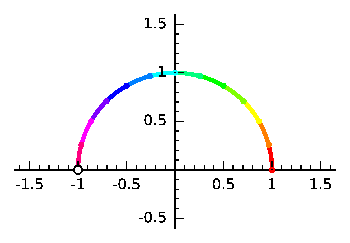
\includegraphics[scale=0.75]{graphics/five_ii_a_unithalfcircle.pdf}}  
\end{equation*}  
\end{frame}




% \section{Angles in plane transformations}
% =============================================
\begin{frame}{Angles}
\ex
This plane transformation.
\begin{equation*} 
  \colvec{x \\ y} \mapsto \colvec{2x \\ 2x+2y}
\end{equation*}
is a skew.
\begin{equation*}
  \vcenteredhbox{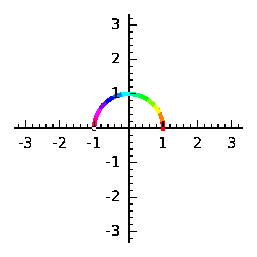
\includegraphics[scale=.75]{graphics/five_ii_a_skew1.pdf}}
  \quad\rightarrow\quad
  \vcenteredhbox{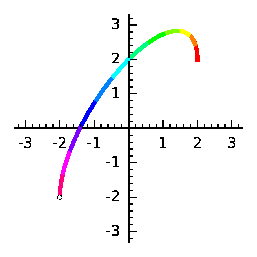
\includegraphics[scale=.75]{graphics/five_ii_a_skew2.pdf}}
\end{equation*}
\pause
As we move through the unit half circle on the left, the 
transformation has varying effects on the vectors.
The dilation vary,
that is, different vectors get their length multiplied by different factors, 
and they are turned through varying angles.
The next slide gives examples.  
\end{frame}
\begin{frame}
The prior slide's vector from the left shown in red
is dilated by a factor of $2\sqrt{2}$ and rotated counterclockwise 
by $\pi/4\approx0.78$~radians.
\begin{equation*}
  \colvec{1 \\ 0}\mapsto \colvec{2 \\ 2}
  \qquad
  \vcenteredhbox{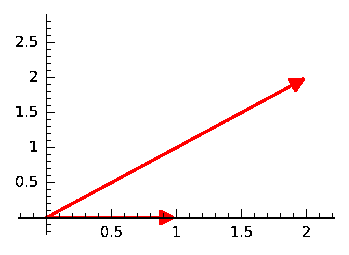
\includegraphics[scale=.75]{graphics/five_ii_a_skew3.pdf}}
\end{equation*}
The orange vector
is dilated by a factor of $2\sqrt{\cos^2(\pi/6)+1}=\sqrt{7}$ and rotated 
by about $0.48$~radians.
\begin{equation*}
  \colvec{\cos(\pi/6) \\ \sin(\pi/6)}\mapsto \colvec{2\cos(\pi/6) \\ 2\cos(\pi/6)+2\sin(\pi/6)}
  \qquad
  \vcenteredhbox{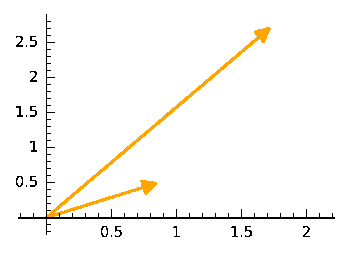
\includegraphics[scale=.75]{graphics/five_ii_a_skew4.pdf}}
\end{equation*}
\end{frame}

\begin{frame}
Here the horizontal axis is the angle of 
vectors from the upper half unit circle.
The vertical axis is
the angle through which the transformation roatates that vector.  
\begin{equation*}
  \colvec{x \\ y}\mapsto \colvec{2x \\ 2x+2y}
  \qquad
  \vcenteredhbox{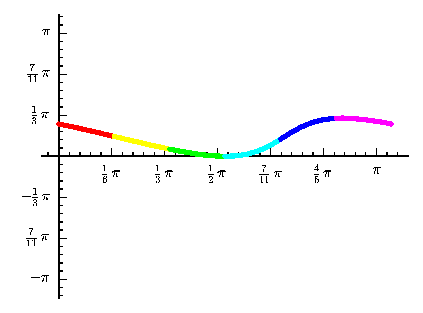
\includegraphics{graphics/five_ii_a_skew5.pdf}}
\end{equation*}
The rotation angle of interest is~$0$~radians, here achieved 
by some green vector.
\end{frame}


\begin{frame}{An alternative definition}
A nonzero 
vector that is rotated through an angle of $0$~radians or of $\pi$~radians
is an \alert{eigenvector}.
The factor by which it is dilated is its \alert{eigenvalue}.    
(By definition, we take the angle of rotation to be in the range
$[0\,\ldots\,2\pi)$.)
\end{frame}



%................
% diagonal
\begin{frame}
\ex
The plane transformation
\begin{equation*} 
  \colvec{x \\ y} \mapsto \colvec{-x \\ 2y}
\end{equation*}
represented with respect to the standard bases by a diagonal matrix
\begin{equation*}
  \begin{mat}
    -1  &0  \\
     0  &2
  \end{mat}
\end{equation*}
has this simple action on the upper half unit circle.
\begin{equation*}
  \vcenteredhbox{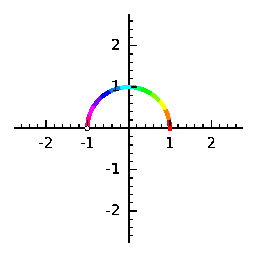
\includegraphics[scale=.75]{graphics/five_ii_a_diagonal1.pdf}}
  \quad\rightarrow\quad
  \vcenteredhbox{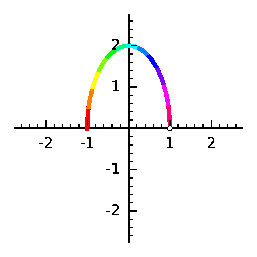
\includegraphics[scale=.75]{graphics/five_ii_a_diagonal2.pdf}}
\end{equation*}
\end{frame}
\begin{frame}
This
plots the angle of each vector in the upper half unit circle
against the angle through which it is rotated.  
\begin{equation*}
  \colvec{x \\ y}\mapsto \colvec{-x \\ 2y}
  \qquad
  \vcenteredhbox{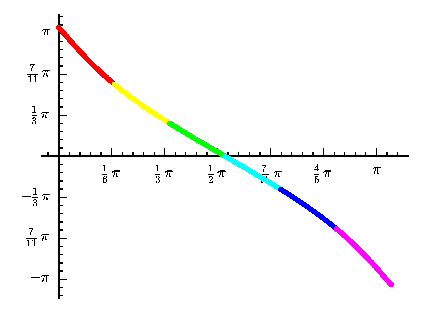
\includegraphics{graphics/five_ii_a_diagonal3.pdf}}
\end{equation*}
One upper-half circle vector is rotated through an angle of $0$~radians,
namely the vector $\vec{e}_2$.
In addition there a vector that is rotated through an angle of 
$\pi$~radians,
namely the vector $\vec{e}_1$.
\end{frame}



%................
% generic
\begin{frame}
\ex
This generic plane transformation
\begin{equation*} 
  \colvec{x \\ y} \mapsto \colvec{x+2y \\ 3x+4y}
\end{equation*}
has this action on the upper half unit circle.
\begin{equation*}
  \vcenteredhbox{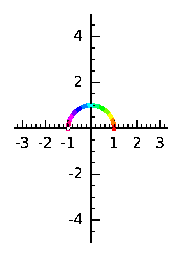
\includegraphics[scale=.75]{graphics/five_ii_a_generic1.pdf}}
  \quad\rightarrow\quad
  \vcenteredhbox{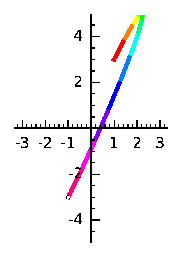
\includegraphics[scale=.75]{graphics/five_ii_a_generic2.pdf}}
\end{equation*}
\end{frame}
\begin{frame}
Plotting the angle of each vector in the upper half unit circle
against the angle through which it is rotated  
\begin{equation*}
  \colvec{x \\ y}\mapsto \colvec{x+2y \\ 3x+4y}
  \qquad
  \vcenteredhbox{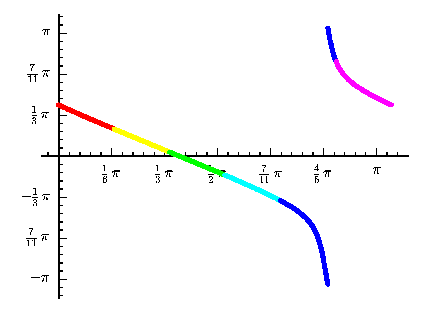
\includegraphics{graphics/five_ii_a_generic3.pdf}}
\end{equation*}
gives that one vector gets a rotation of $0$~radians, while another
gets a rotation of $\pi$~radians.
\end{frame}


% Orange vector calculations
% sage: 2*((cos(pi/6))^2+1)^(1/2)
% sqrt(7)
% sage: v=vector(RR,[cos(pi/6), sin(pi/6)])
% sage: v
% (0.866025403784439, 0.500000000000000)
% sage: M=matrix(RR, [[2,0], [2,2]])
% sage: M
% [ 2.00000000000000 0.000000000000000]
% [ 2.00000000000000  2.00000000000000]
% sage: M=matrix(RR, [[2,2], [0,2]])
% sage: M
% [ 2.00000000000000  2.00000000000000]
% [0.000000000000000  2.00000000000000]
% sage: w=v*M
% sage: w
% (1.73205080756888, 2.73205080756888)
% sage: arccos((w*v)/(w.norm()*v.norm()))
% 0.482170608511459



%...........................
% \begin{frame}g
% \ExecuteMetaData[../gr3.tex]{GaussJordanReduction}
% \df[def:RedEchForm]
% 
% \end{frame}
\end{document}
